\documentclass[11pt,c,compress,UTF8]{ctexbeamer}
\usepackage{ctex}
\usetheme{AnnArbor}
\usecolortheme{dolphin}
\usefonttheme{serif}

\title{Julia 集的分析和探索}
\author{杨钧尹}
\institute{浙江大学 数学科学学院}

\begin{document}

\thispagestyle{empty}   %使封面没有导航条
\maketitle

\section{引言}

% Page1
\begin{frame}
\frametitle{引言:从分形理论说起} 
\begin{figure}[htbp]
\centering
\begin{minipage}{0.3\linewidth}
\centering
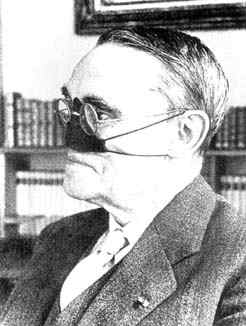
\includegraphics[width = 2.2cm]{./images/julia.jpg}
\caption{\small Gaston Maurice Julia}
\end{minipage}\hfill
\begin{minipage}{0.3\linewidth}
\centering
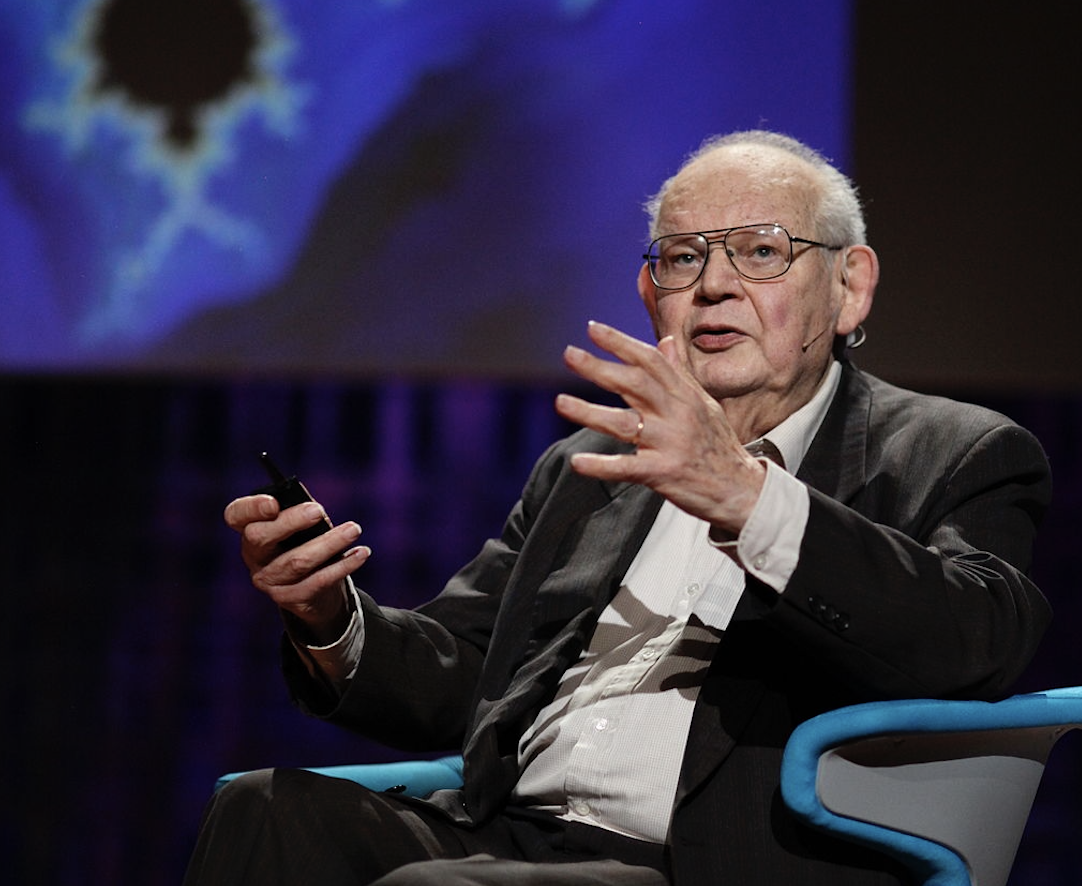
\includegraphics[width = 3.5cm]{./images/mandelbort.png}
\caption{\small Benoit B. Mandelbrot}
\end{minipage}\hfill
\begin{minipage}{0.35\linewidth}
\centering

\includegraphics[width = 2.85cm]{./images/julia_set_example.png}
\caption{\small $c=−0.4+0.6i$的例子}
\end{minipage}
\end{figure}
\end{frame}

\section{理论}

% page2
\subsection{定义}
\begin{frame} 
\frametitle{基本定义}
\begin{block}{}
        这是一个区块
\end{block}
\begin{description}
\item[First Item] Description of first item
\item[Second Item] Description of second item
\item[Third Item] Description of third item
\item[Forth Item] Description of forth item
\end{description}
\end{frame}

% page3
\subsection{特性}
\begin{frame} 
\frametitle{基本定义}
\begin{block}{}
        这是一个区块
\end{block}
\begin{description}
\item[First Item] Description of first item
\item[Second Item] Description of second item
\item[Third Item] Description of third item
\item[Forth Item] Description of forth item
\end{description}
\end{frame}

\section{算法}

% page4
\begin{frame} 
\frametitle{近似算法} 
\begin{itemize} 
 \item 基本无害的计量经济学
 \item 基本有用的计量经济学 
 \item 因果推断实用计量方法
 \item 精通计量:从原因到结果的探寻之旅 
\end{itemize} 
\end{frame}

% page5
\subsection{定义}
\begin{frame} 
\frametitle{基本定义}
\begin{block}{}
        这是一个区块
\end{block}
\begin{description}
\item[First Item] Description of first item
\item[Second Item] Description of second item
\item[Third Item] Description of third item
\item[Forth Item] Description of forth item
\end{description}
\end{frame}

% page6
\subsection{定义}
\begin{frame} 
\frametitle{基本定义}
\begin{block}{}
        这是一个区块
\end{block}
\begin{description}
\item[First Item] Description of first item
\item[Second Item] Description of second item
\item[Third Item] Description of third item
\item[Forth Item] Description of forth item
\end{description}
\end{frame}

% page7
\subsection{定义}
\begin{frame} 
\frametitle{基本定义}
\begin{block}{}
        这是一个区块
\end{block}
\begin{description}
\item[First Item] Description of first item
\item[Second Item] Description of second item
\item[Third Item] Description of third item
\item[Forth Item] Description of forth item
\end{description}
\end{frame}

% page8
\subsection{定义}
\begin{frame} 
\frametitle{基本定义}
\begin{block}{}
        这是一个区块
\end{block}
\begin{description}
\item[First Item] Description of first item
\item[Second Item] Description of second item
\item[Third Item] Description of third item
\item[Forth Item] Description of forth item
\end{description}
\end{frame}

\end{document}